\documentclass{article}
% Packages
\usepackage{graphicx} % Required for inserting images
\usepackage[hidelinks]{hyperref}
\usepackage[dvipsnames]{xcolor} % Custom colors
\usepackage{listings}
\usepackage{amsmath} % For mathematical expressions
\usepackage{amsfonts}
\usepackage{float}

\usepackage{indentfirst}
\usepackage{setspace}
\usepackage{titlesec}
\usepackage{enumitem}
\usepackage{lipsum} % for dummy text

% Colors
\definecolor{sectionblue}{RGB}{25,50,80}
\definecolor{numberbg}{RGB}{25,50,80}
\definecolor{skyblue}{RGB}{135,206,235}

\usepackage{tcolorbox}
\tcbset{
    colback=gray!10,       % Light gray background (like your footer)
    colframe=sectionblue,  % Frame color matches your section numbering
    boxrule=0.5mm,         % Keeps the thin border
    sharp corners,         % Maintains sharp edges
    width=\textwidth,      % Full text width
    fonttitle=\bfseries,   % Bold title if used
    coltitle=sectionblue   % Title text color (if applicable)
}

% Custom section style
\titleformat{\section}
{\normalfont\large\color{sectionblue}\itshape}
{\color{white}
 \setlength{\fboxsep}{4pt}
 \colorbox{numberbg}{\hspace{10pt}\textcolor{white}{\textbf{\thesection}}\hspace{10pt}}
}
{0.1 em}
{}

% Custom subsection style
\titleformat{\subsection}
{\normalfont\large\color{sectionblue}\itshape}
{\color{white}
 \setlength{\fboxsep}{4pt}
 \colorbox{skyblue}{\hspace{10pt}\textcolor{white}{\textbf{\thesubsection}}\hspace{10pt}}
}
{0.1 em} % Space between number box and title
{}

% Custom subsubsection style
\titleformat{\subsubsection}
{\normalfont\normalsize\color{sectionblue}\itshape}
{\color{white}
 \setlength{\fboxsep}{3pt}
 \colorbox{skyblue!70!sectionblue}{\hspace{8pt}\textcolor{white}{\textbf{\thesubsubsection}}\hspace{8pt}}
}
{0.1 em}
{}

% Margins
\usepackage[a4paper, top=2cm, bottom=2.5cm, left=2.5cm, right=2.5cm]{geometry}

% Page number to bottom right
\usepackage{fancyhdr}
\pagestyle{fancy}
\fancyhf{} % clear all header and footer fields
%\fancyfoot[R]{\thepage} % Right side of the footer

\fancyfoot[R]{\rule{\textwidth}{0.5pt}\\ \textcolor{sectionblue}{\textbf{Luis Márquez - Luis Jiménez - Fernando López - Diego Lozoya}} \textbar\ \textcolor{sectionblue}{\textbf{Quantitative Finance}} \quad \colorbox{sectionblue}{\textcolor{white}{\thepage}}}

\renewcommand{\headrulewidth}{0pt} % Optional: remove header line
\renewcommand{\footrulewidth}{0pt} % Optional: remove footer line

\begin{document}

\begin{titlepage}
    \centering
    % TITLE
    {\Huge \textcolor{NavyBlue}{\textbf{A Quantitative Approach to Risk Management in Option Selling}} \par}
    \vspace{0.75cm}

    
\includegraphics[width=0.5\textwidth]{images/ITESOlogo.png}\vspace{0.1cm}

    
\includegraphics[width=0.75\textwidth]{images/FEOFlogo.png}\vspace{0.1cm}
    
    % AUTHORS
    {\Large
    \textcolor{RoyalBlue!60!gray}{Authors:}\\
    \textcolor{RoyalBlue!60!gray}{ }\\
    \textcolor{RoyalBlue!60!gray}{Luis Fernando Márquez Bañuelos}\\
    \textcolor{RoyalBlue!60!gray}{Luis Eduardo Jiménez del Muro}\\
    \textcolor{RoyalBlue!60!gray}{Fernando López Coronado}\\
    \textcolor{RoyalBlue!60!gray}{Diego Lozoya Morales}
    \par}

    % PROFESSOR
    {\Large
    \textcolor{RoyalBlue!60!gray}{ }\\
    \textcolor{RoyalBlue!60!gray}{Professor:}\\
    \textcolor{RoyalBlue!60!gray}{ }\\
    \textcolor{RoyalBlue!60!gray}{José Mario Zárate Carbajal}
    \par}

    \vfill

    % DATE
    {\large \textcolor{SkyBlue}{November 18, 2025}}
\end{titlepage}

\onehalfspacing

\tableofcontents
\thispagestyle{fancy}

\newpage

\section{Presentation}

Financial Engineering Options Fund (FEOF) is an option-focused hedge fund founded by financial engineers and is specialized in generating income through option-based strategies. In this case, Apple Inc. (AAPL) options were used to manage the resulting risk using the Greek option. In this project, we assume the role of its risk-management team and design a complete hedging framework for one specific underlying: AAPL. The fund’s business model is to collect option premia by writing calls and to protect its capital through dynamic hedging strategies based on Delta and higher-order Greeks. Our slogan “Engineering Consistent Performance” shows our commitment to transform market volatility into opportunities.

At the beginning of the investment horizon (September 2nd), the fund sells a portfolio of 10 call options on AAPL with the same maturity but different strike prices. To comply with the requirements of the case, the portfolio is constructed with 5 in-the-money (ITM) options and 5 out-of-the-money (OTM) options, all written at time zero. The premium received from the sale of these contracts represents the initial source of revenue for the strategy, while the potential obligation to deliver the shares at maturity represents the main source of risk.

The objective of this work is to evaluate how different hedging policies affect the distribution of profits and losses (PnL) of the fund. Specifically, we compare three situations: a baseline strategy without hedging, a Delta-only hedging strategy, and a Delta–Gamma hedging strategy, all implemented in the same option portfolio and over the same time period. For each case, we incorporate realistic elements, such as transaction costs when trading the underlying stock and the use of implied volatility extracted from market option prices.

From a strategic perspective, this work illustrates how an options-specialized investment firm can structure and manage a call-writing program on AAPL using standard quantitative tools. From a commercial perspective, it highlights how Greek-based hedging supports a more attractive and stable PnL profile for all clients that seek systematic income with controlled risk.

\newpage

\section{Theory}

\subsection{Usage of Greeks in Hedging}

In derivative markets, traders use Greeks to quantify the sensitivity of an option’s price to changes in the underlying variables. Because option values are nonlinear functions of the underlying asset, effective hedging requires understanding how the option reacts to price movements, time decay, volatility changes, and interest rate effects. Market makers, risk managers, and quantitative traders construct portfolios that are neutral with respect to certain Greeks to reduce risk and stabilize PnL under different market conditions.

\subsection{Implied Volatility Meaning}

One of the most important concepts behind Greek-based hedging is implied volatility. Implied volatility is the volatility level that, when inserted into an option pricing model (such as Black-Scholes), produces the market price of the option. Unlike historical volatility, implied volatility is forward-looking and reflects the market’s expectations and uncertainty about future price movements. It also represents the “price” of risk in the options market—higher implied volatility leads to more expensive option premiums. Implied volatility is central to vega hedging, volatility trading, and strategies involving volatility arbitrage.

\subsection{First-Order Greeks}

\subsubsection{Important Variables}

Financial Call form:

$$
f_t = S_t N(-d_1) - Ke^{-r(T-t)} N(-d_2)
$$

$d_1 \text{and } d_2$:

$$
d_1 = \frac{\ln \left({\frac{S_t}{K}} \right) + \left(r + \frac{\sigma^2}{2} \right)(T-t)}{\sigma \sqrt{T-t}}
$$

$$
d_2 = \frac{\ln \left({\frac{S_t}{K}} \right) + \left(r - \frac{\sigma^2}{2} \right)(T-t)}{\sigma \sqrt{T-t}}
$$

$$
d_2 = d_1 - \sigma \sqrt{T-t}
$$

Normal distribution:

$$
N(x) = \int_{-\infty}^{z_i} \frac{e^{-\frac{1}{2}(x)^2}}{\sqrt{2 \pi}} \ dz
$$

Calculating derivatives:

$$
\frac{\partial N(x)}{\partial x} = \frac{e^{-\frac{1}{2}(x)^2}}{\sqrt{2 \pi}} = N'(x)
$$

$$
\frac{\partial^2 N(x)}{\partial x^2} = -x N'(x) = N''(x)
$$

Where:

\begin{itemize}
    \item $S_t$: Underlying asset price
    \item $K$: Strike price
    \item $r$: Risk-free rate
    \item $\sigma$: Volatility
    \item $T-t$: Remaining time until maturity
\end{itemize}

\subsubsection{Delta $\Delta$}

$$
\Delta = \frac{\partial U_t}{\partial S_t} = N(d_1)
$$

Delta measures how much the option price changes for a small change in the underlying asset price

\subsubsection{Gamma $\Gamma$}

$$
\Gamma = \frac{\partial^2 U_t}{\partial S_t^2} = \frac{\partial \Delta}{\partial S_t} = \frac{N'(d_1)}{S_t \sigma \sqrt{T-t}}
$$

Gamma measures how much delta changes as the underlying price changes (curvature). High gamma means delta is highly sensitive; positions require more frequent rebalancing.

\subsubsection{Vega $\nu$}

$$
\nu = \frac{\partial U_t}{\partial \sigma} = \sqrt{T-t} S_t N'(d_1)
$$

Vega measures how much the option value changes with a 1\% change in volatility.

\subsubsection{Theta $\Theta$}

$$
\theta = - \frac{\partial U_t}{\partial \tau} = - \frac{1}{2}S_t N'(d_1) \frac{\sigma}{\sqrt{\tau}} - r k e ^{-r\tau} N(d_2)
$$

Theta measures the rate at which an option loses value as time passes (“time decay”).

\subsubsection{Rho $\rho$}

$$
\rho = \frac{\partial U_t}{\partial r} = (T-t) k e^{-r(T-t)} N(d_2)
$$

Rho measures the change in option value due to a change in interest rates.

\newpage

\section{Data Prepossessing \& Parameters}

The underlying asset selected for this strategy is Apple Inc., one of the most actively traded equities in the U.S. market and a highly liquid underlying for options analysis. The dataset consists of options information collected over a period of approximately seven weeks, spanning from September 2nd to October 30th. During this interval, a total of 14 observations were recorded, each representing a snapshot of the relevant option parameters at a given date.

To ensure consistency across all calculations, a constant risk-free interest rate of 3.82\% was adopted. This fixed rate was selected for analytical convenience and reflects prevailing market conditions during the period of study. Using this risk-free rate, together with the strike price, underlying price, time to maturity, and market premium of each option, the implied volatility was computed for every sample. This allowed us to derive a volatility measure consistent with market pricing and suitable for subsequent hedging analysis within the strategy. In order to do the hedging analysis all greeks were computed.

Whenever a hedging strategy requires trading the underlying stock, we apply a proportional transaction cost of 0.5\% on the traded notional value, as specified in the case. This cost is included in the PnL of the delta and delta–gamma hedging strategies each time the hedge is rebalanced.

In line with the case description, the option portfolio is composed of 10 call contracts on AAPL, all with the same maturity date. At the writing date (September 2nd), these contracts are selected so that 5 of them are in-the-money (ITM) and the remaining 5 are out-of-the-money (OTM). This construction satisfies the requirement of working with 10 calls, 5 ITM and 5 OTM, all written at time zero.

Finally, the dataset was refined to include only 10 strike prices per observation date. A sample of the resulting filtered dataset is shown below:

\begin{figure}[h!]
    \centering
    \includegraphics[width=1\textwidth]{images/DataSample.png}
\end{figure}

\newpage

\section{Research \& Methodology}

\subsection{Underlying Asset}

Apple Inc. is a global technology company recognized for its leadership in consumer electronics, software, and digital services. Founded in 1976 and headquartered in Cupertino, California, Apple has built a diversified ecosystem anchored by its flagship products such as the iPhone, iPad, Mac, Apple Watch, and AirPods. The company complements its hardware portfolio with a robust suite of software platforms—including iOS, macOS, and watchOS—and an expanding range of high-margin services such as the App Store, Apple Music, iCloud, Apple TV+, and Apple Pay.

Apple operates under a vertically integrated business model that emphasizes tight control over design, hardware, and software, enabling differentiated user experiences and strong customer loyalty. Its financial performance is characterized by substantial revenue generation, healthy operating margins, and consistent cash flow supported by global brand strength and a broad installed base of active devices. As one of the world’s largest publicly traded companies by market capitalization, Apple plays a significant role in both consumer technology trends and global equity markets, making it a highly relevant and liquid underlying asset for financial analysis and trading strategies.

\subsection{Methodology}

Every strategy starts on September the 2nd and ends on November the 20th (a day before maturity). The Spot price of November the 20th is assumed to be \$271.40, the same as the last one recovered on October the 30th

\subsubsection{No Hedging}

At the beginning of the evaluation period (September 2nd), one option at each selected strike price was sold, and the corresponding premiums were collected. The total premium received amounted to \$135.62, which was subsequently invested at the risk-free interest rate. By the end of the period (November 20th), this investment yielded \$136.74.

At maturity, the spot price reached \$271.40, resulting in all options finishing in-the-money. Consequently, the short option positions were exercised, requiring a total payout of \$2,714 to settle the obligations, while the options delivered only \$2,320 in proceeds. After accounting for the premiums and accumulated interest, the strategy resulted in a net loss of \$257.26.

\subsubsection{Delta Hedging}

In the Delta Hedge strategy, the same 10 options, each corresponding to a different strike, were sold on September 2nd, generating a total premium of \$135.62. This amount was invested at the risk-free interest rate, yielding \$136.74 by November 20th.

At every time step during the hedging period, the delta of each option was computed. The individual deltas were then aggregated to obtain the overall portfolio delta. Changes in this aggregated delta determined the adjustments required in the underlying asset position to maintain the hedge. Specifically, the differential in delta between periods indicated the quantity of the underlying that needed to be bought or sold.

As in the no-hedge scenario, all 10 options expired in-the-money and were exercised. Under the Delta Hedge strategy, the total cost to settle the exercised positions amounted to \$2,249.04, while the options themselves generated proceeds of \$2,320. After incorporating the premium received, accumulated interest, and transaction costs, the strategy produced a net profit of \$207.70.

\subsubsection{Delta-Gamma Hedging}

The same 10 options, each corresponding to a different strike, were sold on September 2nd, generating a total premium of \$135.62. This amount was invested at the risk-free interest rate, yielding \$136.74 by November 20th.

The delta–gamma hedging approach extends this methodology by incorporating sensitivity to curvature in the option portfolio. To determine when a gamma adjustment should be triggered, gamma thresholds were established based on the portfolio’s exposure dynamics rather than arbitrarily chosen levels. As part of this process, different portfolios of ten options were simulated and their corresponding gamma values were computed; based on the distribution of these simulated gammas, the thresholds were set using the 25th percentile for the lower bound and the 75th percentile for the upper bound. This ensured that the thresholds reflected realistic variations in portfolio curvature rather than relying on subjective assumptions.

This approach ensured that rebalancing was performed only when gamma exposure became significant enough to materially impact the hedge relative to transaction costs and overall portfolio sensitivities. Based on this empirical procedure, the upper and lower gamma thresholds were set at 0.102250 and 0.082176, respectively.

At each time step, the portfolio gamma was evaluated and compared to these thresholds. Whenever gamma exceeded the defined limits, a gamma-hedging adjustment was applied in conjunction with the existing delta hedge. Specifically, when the threshold was breached, the delta hedge was scaled by a factor of ±0.1, effectively adjusting the hedge to 1.1 times or 0.9 times the original delta value depending on the direction of the required correction.

With the gamma-adjusted hedging procedure, the total payout required to settle the exercised positions was \$1,987.52, while the option exercises yielded the same \$2,320 in proceeds. After incorporating premiums, accumulated interest, and hedging adjustments, the delta–gamma hedging strategy produced a total profit of \$469.22.

\newpage

\section{Simulations}

To obtain more robust and statistically reliable results, a set of 1,000 Monte Carlo simulations of the spot price was generated using Model 2. This simulation framework allowed the strategy outcomes to be evaluated under a wide range of plausible market scenarios, providing a higher degree of confidence in the comparative performance of each hedging approach. For each simulated path, the same methodology previously described was applied to compute the corresponding profitability.

Model 2:
$$
S_t = S_0 e^{\left(\mu_R - \frac{1}{2}\sigma^2 \right)(T-t)+\sigma \sqrt{T-t}W_1}
$$
Where:

\begin{itemize}
    \item $S_0$: Underlying asset price
    \item $\mu_R$: Annualized expected return of the asset
    \item $\sigma^2$: Annualized variance of the asset returns
    \item $T-t$: Remaining time until maturity
    \item $W_1$: Wiener process distributed as $\mathcal{N} \sim (0,1)$
\end{itemize}

\subsection{No Hedging}

Under the no-hedging strategy, the average PnL across the 1,000 simulations was -\$92.83. The distribution of returns for this strategy is illustrated below:

\begin{figure}[h!]
    \centering
    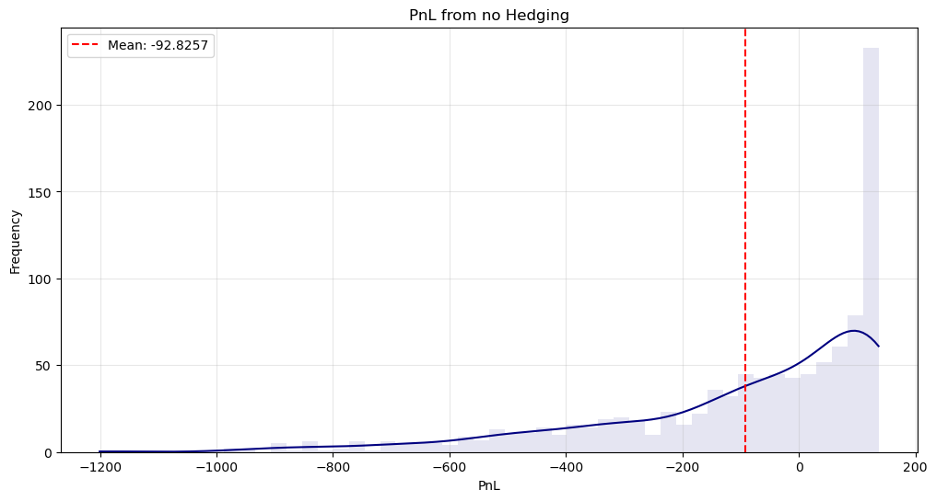
\includegraphics[width=1\textwidth]{images/NoHedgeHist.png}
\end{figure}

The simulation results also indicate that the probability of incurring a loss under the no-hedging strategy is 52.30\%, reflecting nearly an even likelihood of negative performance. Additionally, the 95\% Value at Risk (VaR) for this strategy was estimated at –\$602.49, meaning that with 95\% confidence, the maximum expected loss over the period would not exceed this amount under normal market conditions.

\subsection{Delta Hedging}

Under the Delta hedging strategy, the average PnL across the 1,000 simulations was -\$40.55. The distribution of returns for this strategy is illustrated below:

\begin{figure}[h!]
    \centering
    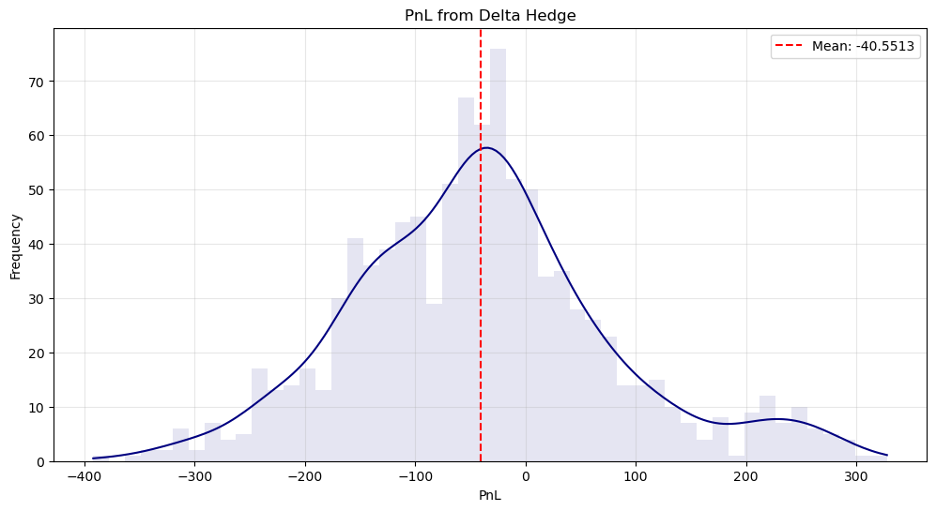
\includegraphics[width=1\textwidth]{images/DeltaHedgeHist.png}
\end{figure}

For the Delta Hedge strategy, the simulation results show a 68.30\% probability of experiencing a loss, indicating that while the hedge reduces tail risk, it increases the likelihood of small negative outcomes due to frequent rebalancing and transaction costs. The 95\% Value at Risk (VaR) for this strategy was estimated at –\$226.74, demonstrating a substantial reduction in downside exposure compared to the no-hedging approach.

\subsection{Delta-Gamma Hedging}

Finally, under the Delta-Gamma hedging strategy, the average PnL across the 1,000 simulations was \$60.69. The distribution of returns for this strategy is illustrated below:

\begin{figure}[h!]
    \centering
    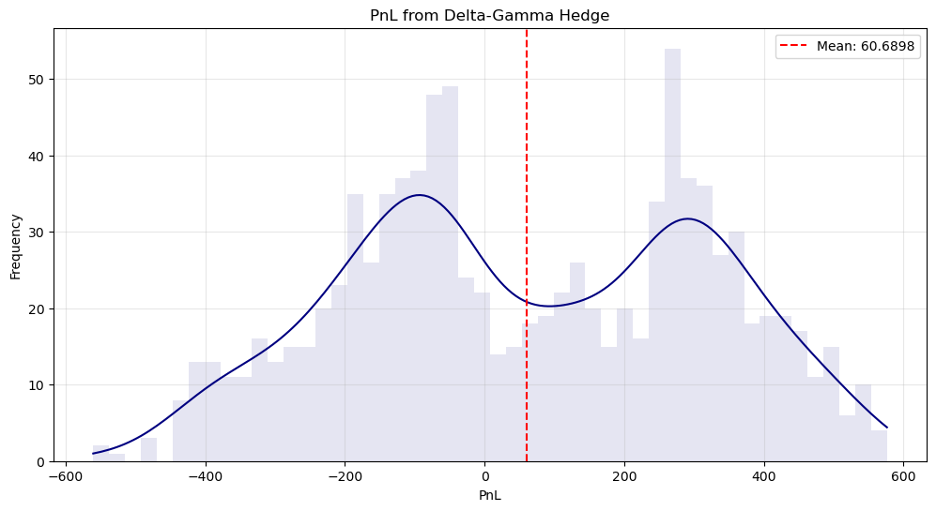
\includegraphics[width=1\textwidth]{images/DeltaGammaHedgeHist.png}
\end{figure}

For the Delta–Gamma Hedge strategy, the probability of incurring a loss falls to 47.40\%, making it the only approach with a loss probability below 50\% in the simulation study. Its 95\% Value at Risk (VaR) is estimated at –\$358.19, indicating a moderate level of downside risk. Although the VaR is not as low as that of the Delta Hedge strategy, the Delta–Gamma approach offers a more balanced trade-off between loss frequency and tail-risk protection.

\subsection{Implied Volatility Analysis}

\begin{figure}[h!]
    \centering
    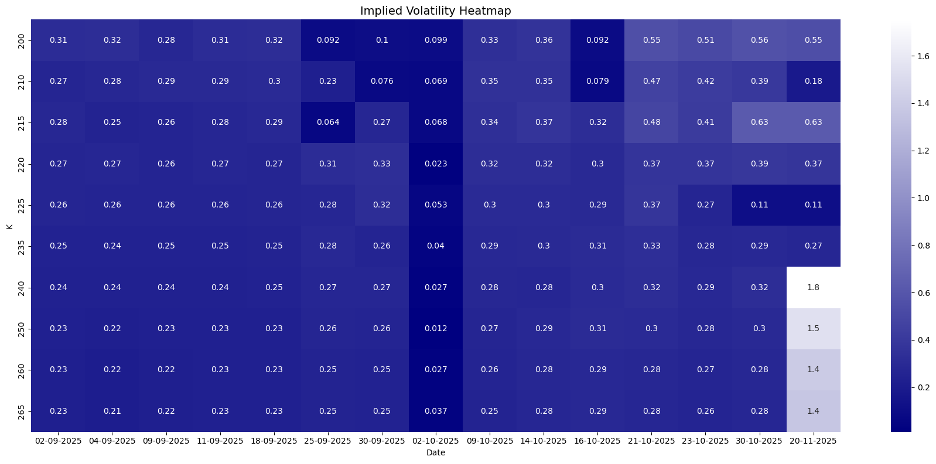
\includegraphics[width=1\textwidth]{images/ImpVolHeatmap.png}
\end{figure}

The implied volatility heatmap provides insight into the market’s evolving expectations of uncertainty throughout the hedging horizon, and this information directly influences the behavior of the simulated PnL distributions. Periods where implied volatility rises, visible in several dates and strikes, reflect higher anticipated variability in future spot prices, which in turn amplifies the dispersion observed in the Monte Carlo simulations. These elevated volatility levels contribute to wider PnL distributions, larger tail values, and more extreme outcomes, particularly evident in the no-hedging and delta-only strategies. Conversely, when implied volatility remains stable or lower, the simulated paths exhibit tighter clusters and reduced tail risk. The delta–gamma hedging strategy benefits the most from these volatility regimes, as its curvature adjustments allow it to better adapt to changes in implied volatility and mitigate the effect of large price swings. Overall, the heatmap serves as a forward-looking indicator that helps explain the shape, spread, and risk characteristics of the simulated PnL distributions across the three strategies.

\newpage

\section{Conclusions}

\begin{figure}[h!]
    \centering
    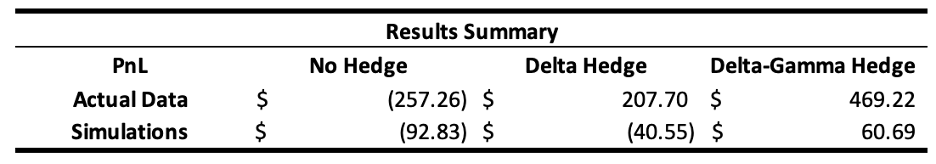
\includegraphics[width=1\textwidth]{images/ResultsSummary.png}
\end{figure}

The results demonstrate the substantial impact that hedging methodology has on the performance and risk profile of an options portfolio. Under actual market data, the no-hedge strategy produced a significant loss, while both hedged strategies generated positive PnL, with the delta–gamma hedge clearly outperforming the delta-only approach. The simulation results present a consistent narrative: although the no-hedge and delta-hedge strategies tend to yield negative expected returns, the delta–gamma hedge maintains a positive average outcome, reinforcing its robustness across a broad range of market scenarios. Overall, the evidence suggests that incorporating second-order sensitivities into the hedging process provides meaningful protection against nonlinear price movements, reduces tail risk, and enhances the stability of returns, making the delta–gamma approach the most effective strategy among the three evaluated.

\newpage

\section{References}

\begin{itemize}
    \item Investopedia. (n.d.). Delta-Gamma Hedging. In Investopedia. Retrieved November 12, 2025, from https://www.investopedia.com/terms/d/deltagamma-hedging.asp 
    \item Investopedia. (n.d.). Delta Hedging. In Investopedia. Retrieved November 12, 2025, from https://www.investopedia.com/terms/d/deltahedging.asp
    \item Investopedia. (n.d.). Implied Volatility (IV). In Investopedia. Retrieved November 12, 2025, from https://www.investopedia.com/terms/i/iv.asp
    \item Investopedia. (n.d.). Getting to Know the Greeks. In Investopedia. Retrieved November 12, 2025, from https://www.investopedia.com/trading/getting-to-know-the-greeks/
    \item Wikipedia. (2024). Greeks (finance). In Wikipedia, The Free Encyclopedia. Retrieved November 12, 2025, from https://en.wikipedia.org/wiki/Greeks\_(finance)
\end{itemize}

\end{document}
